\begin{figure}[htbp]
    \centering
    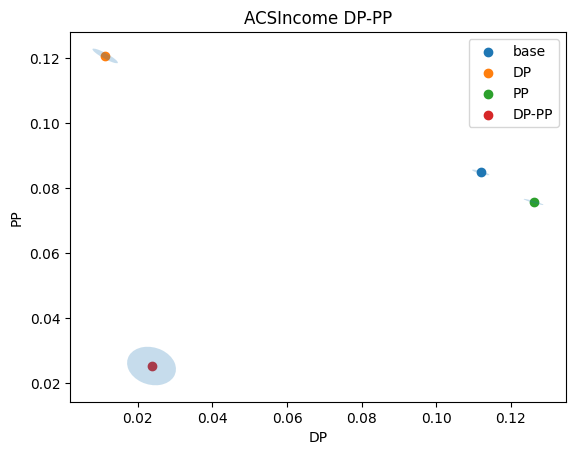
\includegraphics[width=0.8\textwidth]{assets/combined/ACSIncome_DP-PP.png}
    \caption{Violation measures of DP and PP for an unconstrained baseline model, single constrained models and a combined constrained model. Averages were calculated from 5 samples runs.}
    \label{fig:pair1}
\end{figure}



\begin{figure}[htbp]
    \centering
    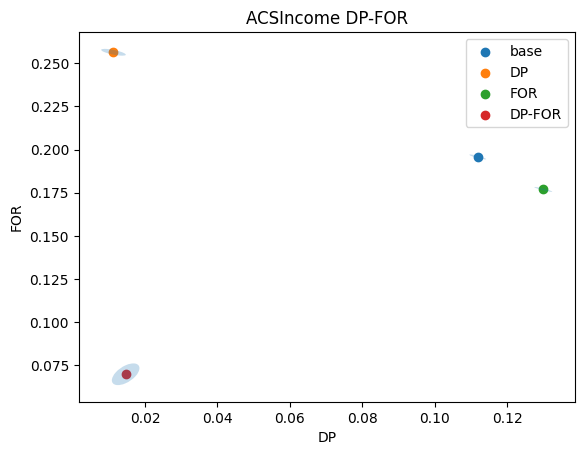
\includegraphics[width=0.8\textwidth]{assets/combined/ACSIncome_DP-FOR.png}
    \caption{Violation measures of DP and FOR for an unconstrained baseline model, single constrained models and a combined constrained model. Averages were calculated from 5 samples runs.}
\end{figure}
    

\begin{figure}[htbp]
    \centering
    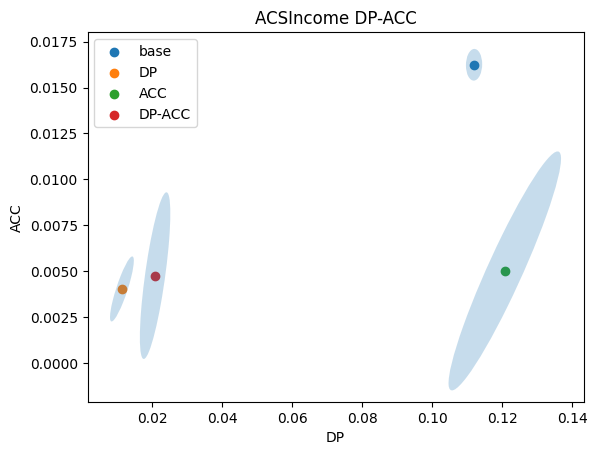
\includegraphics[width=0.8\textwidth]{assets/combined/ACSIncome_DP-ACC.png}
    \caption{Violation measures of DP and ACC for an unconstrained baseline model, single constrained models and a combined constrained model. Averages were calculated from 5 samples runs.}
\end{figure}
    

\begin{figure}[htbp]
    \centering
    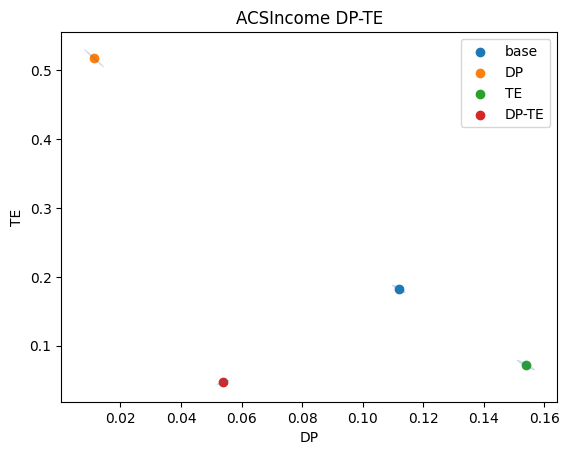
\includegraphics[width=0.8\textwidth]{assets/combined/ACSIncome_DP-TE.png}
    \caption{Violation measures of DP and TE for an unconstrained baseline model, single constrained models and a combined constrained model. Averages were calculated from 5 samples runs.}
\end{figure}
    

\begin{figure}[htbp]
    \centering
    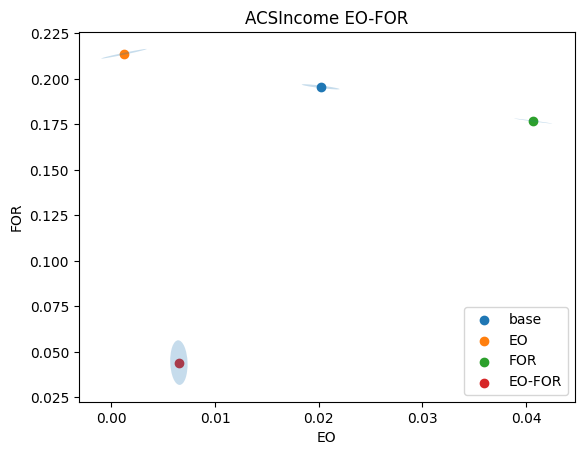
\includegraphics[width=0.8\textwidth]{assets/combined/ACSIncome_EO-FOR.png}
    \caption{Violation measures of EO and FOR for an unconstrained baseline model, single constrained models and a combined constrained model. Averages were calculated from 5 samples runs.}
\end{figure}
    

\begin{figure}[htbp]
    \centering
    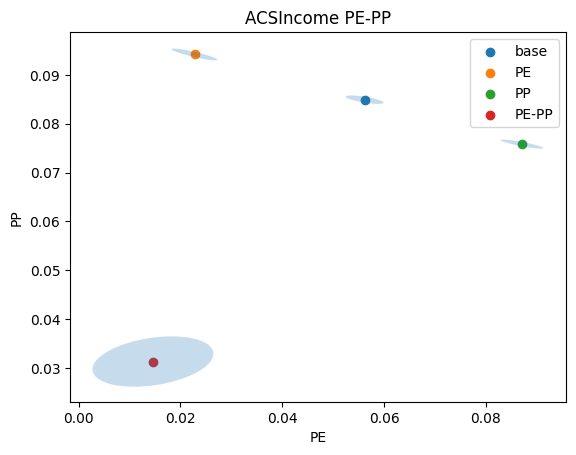
\includegraphics[width=0.8\textwidth]{assets/combined/ACSIncome_PE-PP.png}
    \caption{Violation measures of PE and PP for an unconstrained baseline model, single constrained models and a combined constrained model. Averages were calculated from 5 samples runs.}
\end{figure}
    

\begin{figure}[htbp]
    \centering
    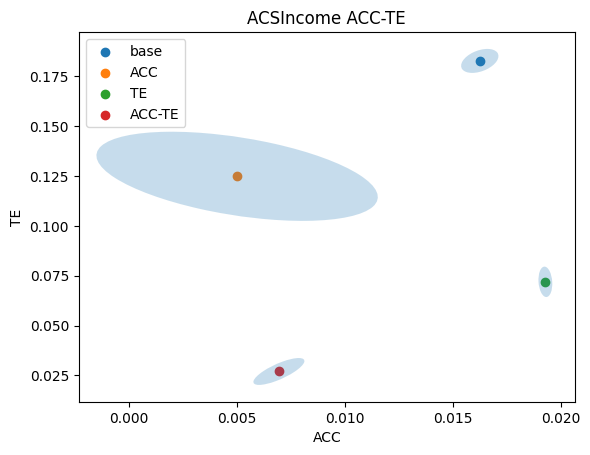
\includegraphics[width=0.8\textwidth]{assets/combined/ACSIncome_ACC-TE.png}
    \caption{Violation measures of ACC and TE for an unconstrained baseline model, single constrained models and a combined constrained model. Averages were calculated from 5 samples runs.}
\end{figure}
    

\begin{figure}[htbp]
    \centering
    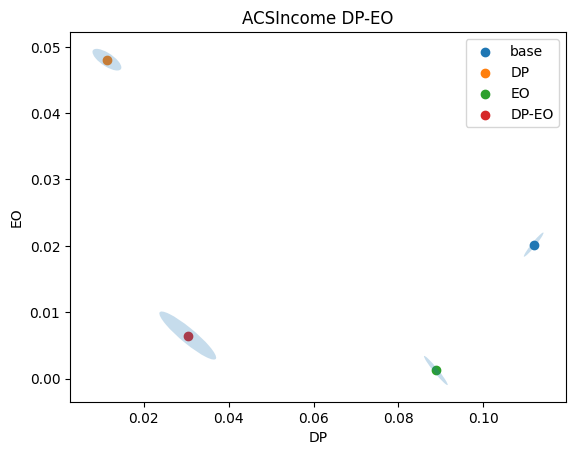
\includegraphics[width=0.8\textwidth]{assets/combined/ACSIncome_DP-EO.png}
    \caption{Violation measures of DP and EO for an unconstrained baseline model, single constrained models and a combined constrained model. Averages were calculated from 5 samples runs.}
\end{figure}
    

\begin{figure}[htbp]
    \centering
    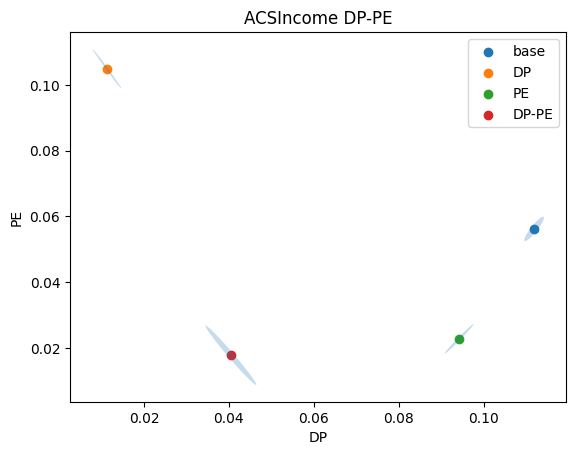
\includegraphics[width=0.8\textwidth]{assets/combined/ACSIncome_DP-PE.png}
    \caption{Violation measures of DP and PE for an unconstrained baseline model, single constrained models and a combined constrained model. Averages were calculated from 5 samples runs.}
\end{figure}
    

\begin{figure}[htbp]
    \centering
    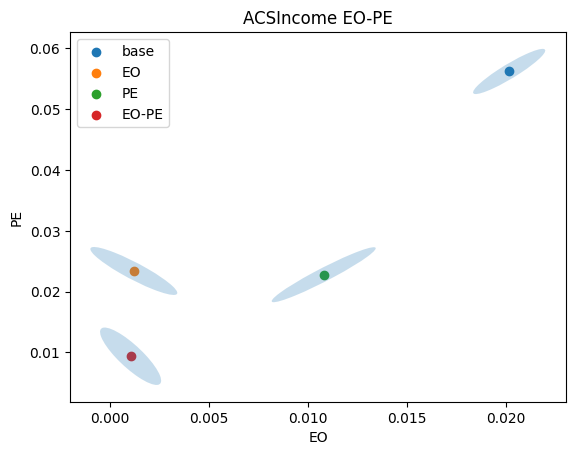
\includegraphics[width=0.8\textwidth]{assets/combined/ACSIncome_EO-PE.png}
    \caption{Violation measures of EO and PE for an unconstrained baseline model, single constrained models and a combined constrained model. Averages were calculated from 5 samples runs.}
\end{figure}
    

\begin{figure}[htbp]
    \centering
    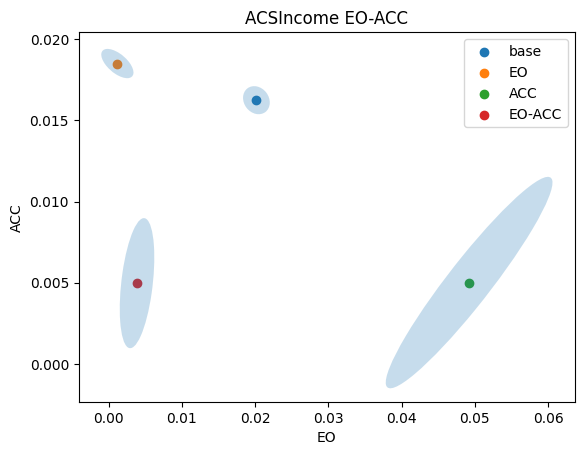
\includegraphics[width=0.8\textwidth]{assets/combined/ACSIncome_EO-ACC.png}
    \caption{Violation measures of EO and ACC for an unconstrained baseline model, single constrained models and a combined constrained model. Averages were calculated from 5 samples runs.}
\end{figure}
    

\begin{figure}[htbp]
    \centering
    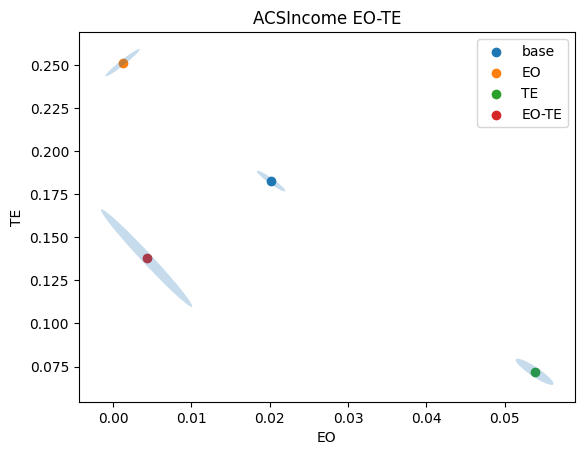
\includegraphics[width=0.8\textwidth]{assets/combined/ACSIncome_EO-TE.png}
    \caption{Violation measures of EO and TE for an unconstrained baseline model, single constrained models and a combined constrained model. Averages were calculated from 5 samples runs.}
    \label{fig:EO-TE}
\end{figure}
    

\begin{figure}[htbp]
    \centering
    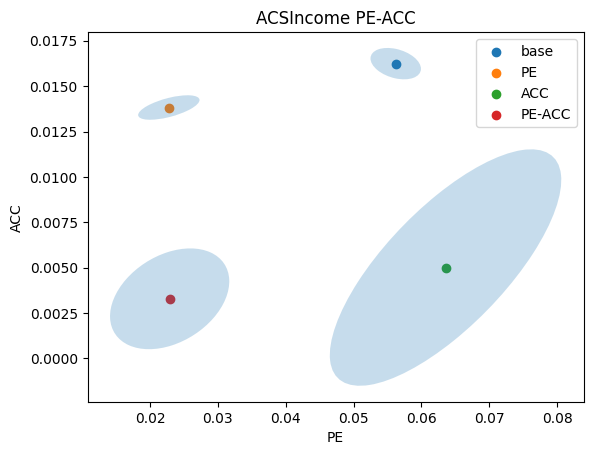
\includegraphics[width=0.8\textwidth]{assets/combined/ACSIncome_PE-ACC.png}
    \caption{Violation measures of PE and ACC for an unconstrained baseline model, single constrained models and a combined constrained model. Averages were calculated from 5 samples runs.}
\end{figure}
    

\begin{figure}[htbp]
    \centering
    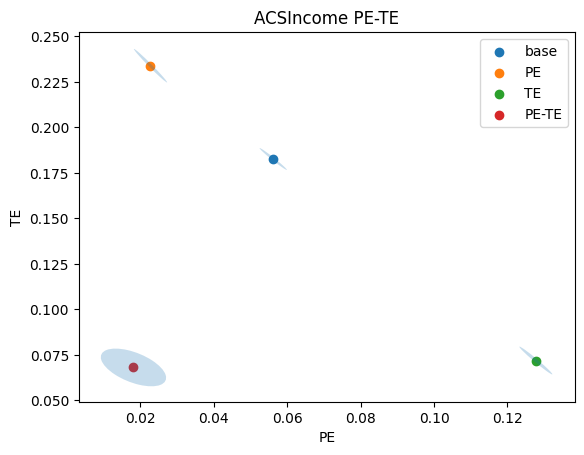
\includegraphics[width=0.8\textwidth]{assets/combined/ACSIncome_PE-TE.png}
    \caption{Violation measures of PE and TE for an unconstrained baseline model, single constrained models and a combined constrained model. Averages were calculated from 5 samples runs.}
\end{figure}
    

\begin{figure}[htbp]
    \centering
    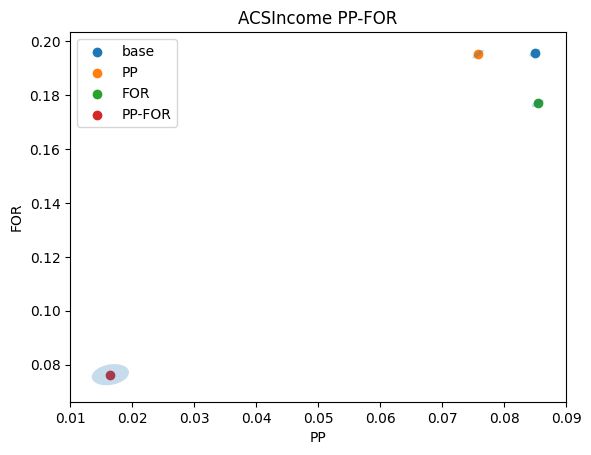
\includegraphics[width=0.8\textwidth]{assets/combined/ACSIncome_PP-FOR.png}
    \caption{Violation measures of PP and FOR for an unconstrained baseline model, single constrained models and a combined constrained model. Averages were calculated from 5 samples runs.}
\end{figure}
    

\begin{figure}[htbp]
    \centering
    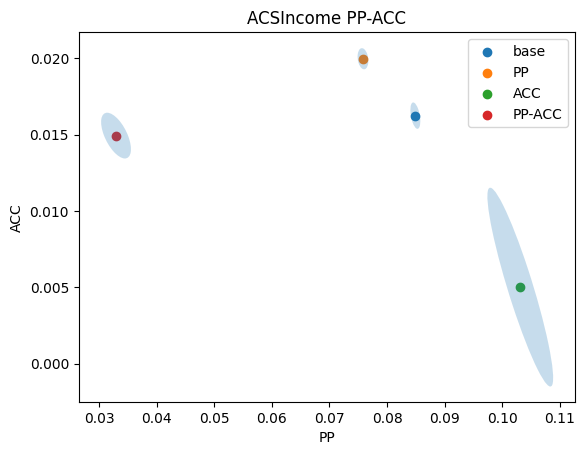
\includegraphics[width=0.8\textwidth]{assets/combined/ACSIncome_PP-ACC.png}
    \caption{Violation measures of PP and ACC for an unconstrained baseline model, single constrained models and a combined constrained model. Averages were calculated from 5 samples runs.}
    \label{fig:PP-ACC}
\end{figure}
    

\begin{figure}[htbp]
    \centering
    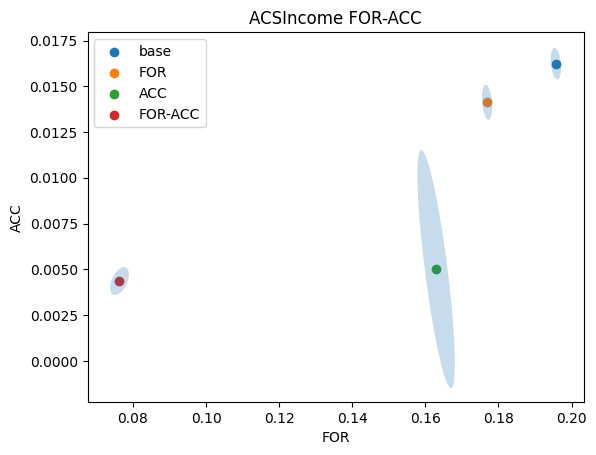
\includegraphics[width=0.8\textwidth]{assets/combined/ACSIncome_FOR-ACC.png}
    \caption{Violation measures of FOR and ACC for an unconstrained baseline model, single constrained models and a combined constrained model. Averages were calculated from 5 samples runs.}
\end{figure}
    

\begin{figure}[htbp]
    \centering
    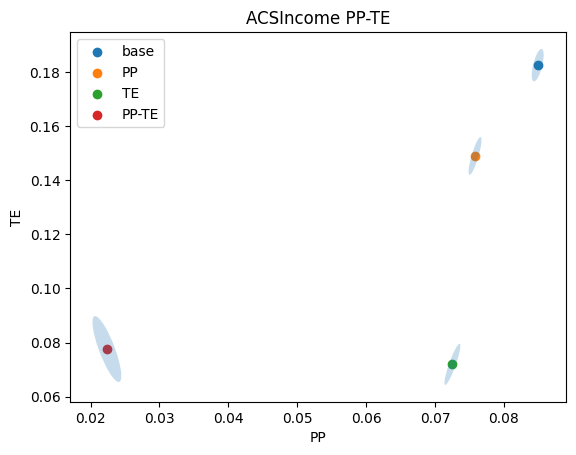
\includegraphics[width=0.8\textwidth]{assets/combined/ACSIncome_PP-TE.png}
    \caption{Violation measures of PP and TE for an unconstrained baseline model, single constrained models and a combined constrained model. Averages were calculated from 5 samples runs.}
\end{figure}
    

\begin{figure}[htbp]
    \centering
    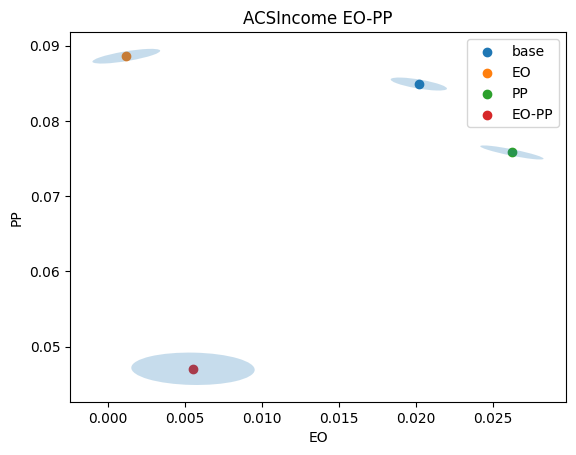
\includegraphics[width=0.8\textwidth]{assets/combined/ACSIncome_EO-PP.png}
    \caption{Violation measures of EO and PP for an unconstrained baseline model, single constrained models and a combined constrained model. Averages were calculated from 5 samples runs.}
\end{figure}
    

\begin{figure}[htbp]
    \centering
    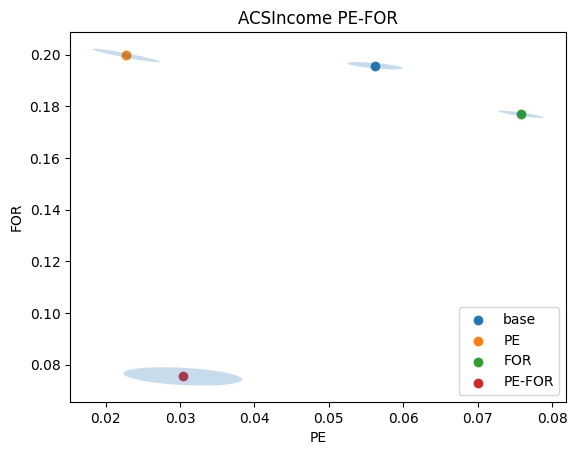
\includegraphics[width=0.8\textwidth]{assets/combined/ACSIncome_PE-FOR.png}
    \caption{Violation measures of PE and FOR for an unconstrained baseline model, single constrained models and a combined constrained model. Averages were calculated from 5 samples runs.}
\end{figure}
    

\begin{figure}[htbp]
    \centering
    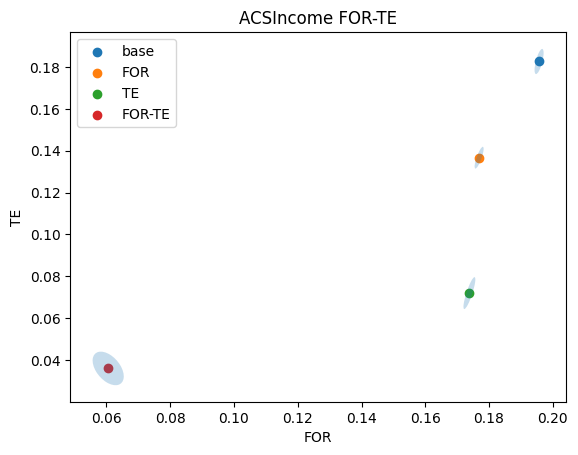
\includegraphics[width=0.8\textwidth]{assets/combined/ACSIncome_FOR-TE.png}
    \caption{Violation measures of FOR and TE for an unconstrained baseline model, single constrained models and a combined constrained model. Averages were calculated from 5 samples runs.}
    \label{fig:pair21}
\end{figure}
